
\section{Introduction}
Ce stage s'inscrit dans le cadre de l'identification des paramètres fonctionnels (\textit{cf.} Section 1.3) visant à analyser le ballast afin de détecter les excès ou les manques de celui-ci. Cette introduction a pour objectif de présenter l'entreprise ainsi que le projet Hyperion (\textit{cf.} Section 1.2), grâce auquel le projet RHEA (\textit{cf.} Section 2) est né, en s'appuyant sur la documentation fournie par Cegelec \cite{Hyperion-interface}. Les objectifs que visa à atteindre ce projet sera également présenter.

\subsection{Présentation de l'Entreprise}

Vinci Energies Belgium est une filiale du groupe VINCI, un leader dans les secteurs de l'industrie, du tertiaire, des infrastructures et de l'ICT. Elle est engagée dans la transformation digitale et la transition énergétique à travers le déploiement de nouvelles technologies pour soutenir ses clients dans la réalisation de leurs projets. À travers ses 15 marques, elle offre des solutions allant de la conception à la réalisation, ainsi que des méthodes d'optimisation pour garantir la réussite de leurs projets. En tant que stagiaire, j'ai été recruté par la marque Cegelec Infra Technics, spécialisée dans l'ingénierie, le développement de logiciels et les technologies pour les projets d'infrastructure. Un contrat CIP (Convention d'Immersion Professionnelle) a été signé pour une durée de 8 mois, avec une charge horaire de 20 heures par semaine, dans le but de me permettre d'acquérir des compétences professionnelles hautement valorisantes. 

\subsection{Hyperion}

Cegelec Infra Technics en collaboration avec ADCIS, une compagnie spécialisée dans la vision par ordinateur et l'intelligence artificielle, a conçu le système Hyperion pour Infrabel dans le but de vérifier les données topographiques du réseau ferroviaire. Ce système utilise des capteurs de vision et de localisation installés sur deux trains de mesure, afin de recueillir des données précises sur l'infrastructure ferroviaire, permettant ainsi une comparaison avec les données réelles existantes. \\

\noindent Le système Hyperion est composé de deux composants.
\begin{itemize}
    \item Une unité d'acquisition embarqué dans le train (\textit{cf.} Figure 1) qui permet d'acquérir des données visuelles telles que les images, les profils du terrain, les nuages de points, ainsi que des données de navigation (\textit{cf.} Figure 2).
        \begin{figure}[H]
            \centering
            \fbox{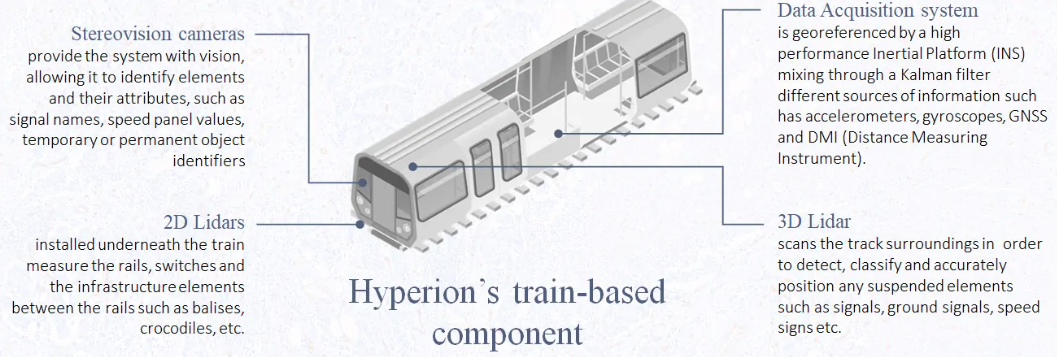
\includegraphics[width=15cm]{images/Hyperion-train-based-system.png}  } 
            \caption{Unité d'acquisition embarquée - ADCIS \cite{Hyperion-Unité}} 
        \end{figure}
        \begin{figure}[H]
            \centering
            \fbox{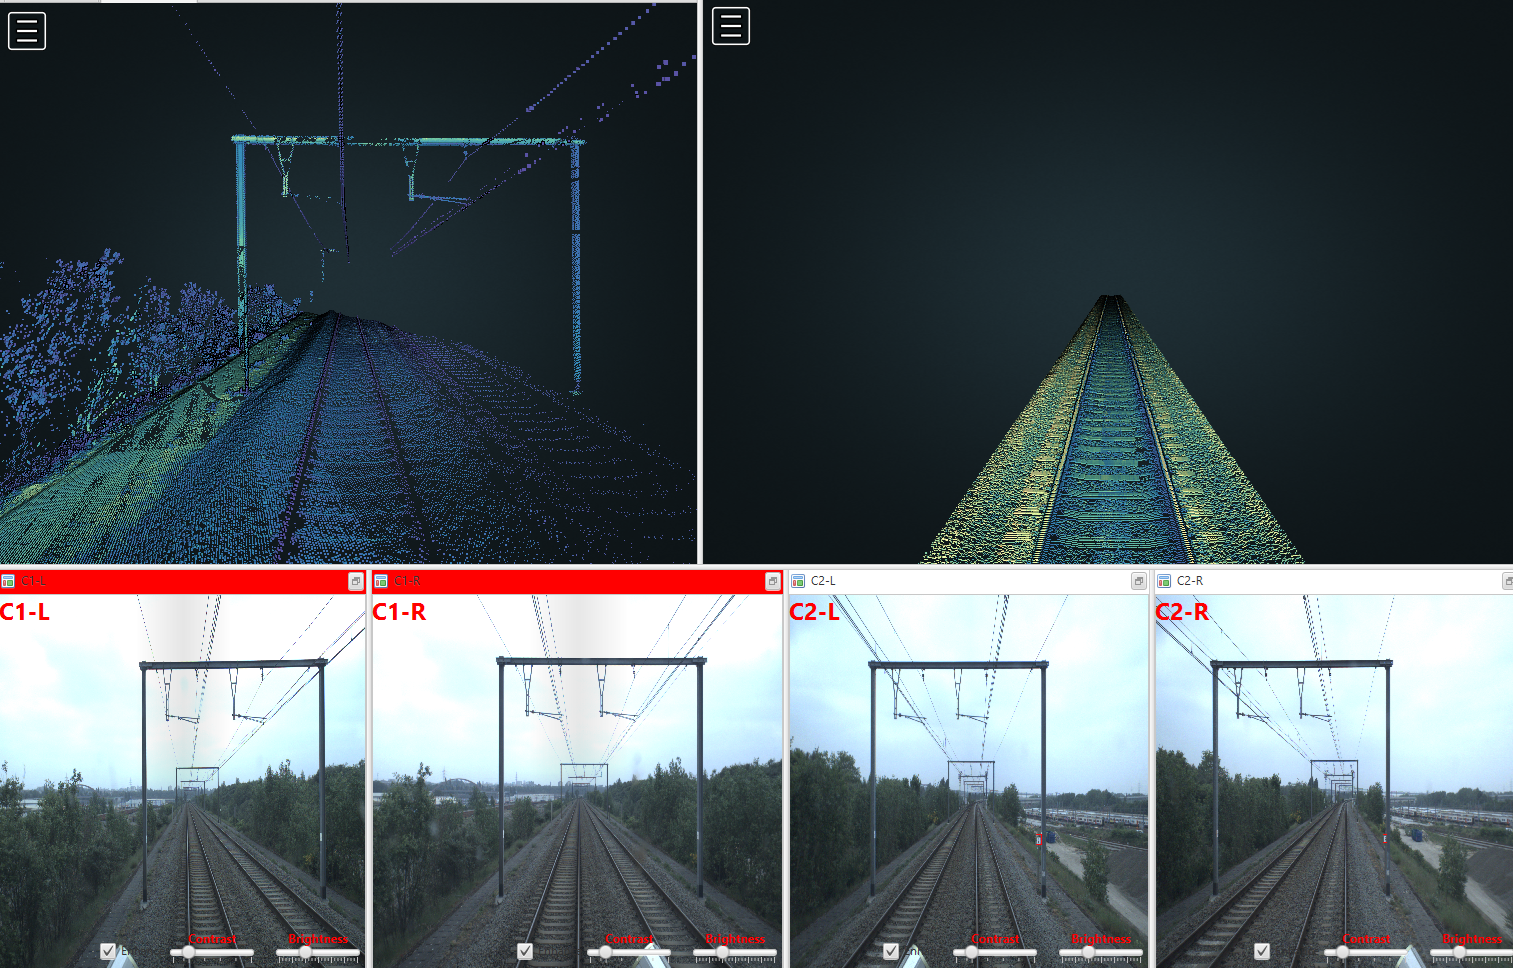
\includegraphics[width=12cm]{images/Hyperion-Interface.png}}   
            \caption{Visualisation dans Hyperion des nuages de points et des images relevés au cours d'une \gls{campagne}.} 
        \end{figure}
    \item 
Un système de reconnaissance et de vérification de la présence des éléments d'infrastructure a été développé à Bruxelles par ADCIS. Ce système consiste à synchroniser les données recueillies par tous les capteurs pendant une campagne, à géolocaliser ces données, à détecter et identifier les éléments ferroviaires, puis à les comparer avec des mesures antérieures (\textit{cf.} Figure 3). 
    
     \begin{figure}[H]
        \centering
        \fbox{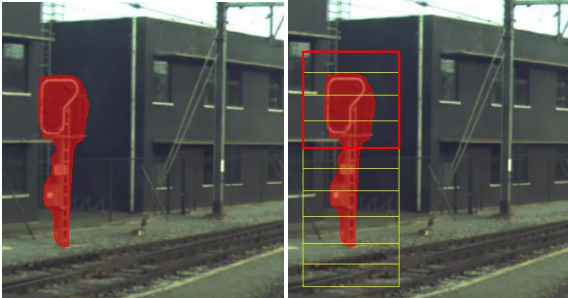
\includegraphics[width=10cm]{images/Hyperion-Identification.png} }  
        \caption{Identification et détection d'un élement ferroviaire - Documentation Cegelec \cite{Hyperion-interface}} 
    \end{figure}   
    
\end{itemize}


\subsection{Objectifs} 

L'objectif du projet est la conception d'un système informatique déstiné à analyser les données collectées par les trains de mesure d'Infrabel (\textit{cf.} Section 1.2), afin de développer un outil de maintenance prédictive du ballast férroviaire (\textit{cf.} Section 2), en se basant sur les paramètres fonctionnels tels que ceux qui suivent.

\begin{itemize}
\item \textbf{La vitesse} du train qui indique la direction de déplacement, soit vers l'avant (positif), soit en marche arrière (négatif). En cas de changement de direction d'un train, un nouveau segment est créé pour éviter la répétition d'une même portion de voie dans un seul segment.

\item \textbf{Le réseau}, qu'il soit un réseau conventionnel ou dédié aux lignes à grande vitesse.

\item \textbf{La structure}, c'est-à-dire les éléments physiques situés à gauche, à droite ou des deux côtés tels qu'un mur, un quai de gare, un pilier en béton, etc.

\item \textbf{La topologie}, il s'agit de la configuration de la proximité d'autres voies dans l'environnement, que ce soit simple ou double.

\item \textbf{La courbe} désigne la forme de la voie, pouvant être droite, courbée ou inclinée.

\item \textbf{Les zones exclues}, ce sont des zones où l'analyse du ballast ne doit pas être réalisée, telles que les ponts, les tunnels, les passages à niveau, les interrupteurs simples, les interrupteurs doubles et les interrupteurs de croisement.

\item \textbf{Les composants de voie} tels que le \gls{crocodile}, l'\gls{ETCS}.

\item \textbf{Les traverses} sont de différents types et peuvent être observés sur le terrain. Elles sont fabriquées en bois ou en acier (WS), ou encore en béton avec différentes formes, telles que les monoblocs (MB3, MB5, etc.) ou les biblocs (BB1, BB2, etc.). \cite{RHEA}
\end{itemize}


\noindent Les paramètres fonctionnels jouent un rôle essentiel dans l'établissement du profil théorique du ballast. Ce profil théorique sert de référence lors de la comparaison avec les données relevées, permettant ainsi de détecter d'éventuels déficits ou excès de ballast.\\

\noindent L'objectif du stage, quant à lui, peut être articulé sur trois points distintcs. 

\begin{itemize}
    \item \textbf{Identification du Type de Traverse de Voie} \\
    Le système vise à mettre en place une technologie permettant l'identification précise du type de traverse. Ces traverses peuvent être en bois, en métal ou en béton, possédant chacune un ensemble de sous-types spécifiques.
    
    \item \textbf{Identification de voies adjacentes à la voie courante} \\
    L'identification de la topologie de la voie est importante, car l'absence de voie à proximité se traduit par la formation d'un épaulement aux extremités du profil de référence, tandis que la présence d'une voie se caractèrise par un profil plat. Les configurations de topologies suivantes doivent être identifiées : simple voie, entre voie - voie à gauche, entrevoie - voie à droite, entrevoie - voies à gauche et droite. 

    \item \textbf{Localisation de la végétation} \\
    En complément, le système pourrait intégrer une fonctionnalité de détection de la végétation pour compenser le volume supplémentaire généré par la forme de la végétation lors de l'analyse du ballast. Cette fonctionnalité serait également utilisée afin d'optimiser la gestion de la végétation le long des voies ferroviaires. Actuellement, l'identification des zones nécessitant un entretien de la végétation se fait par relevé pédestre. L'objectif est de mettre en place un processus automatisé capable de cartographier les endroits présentant de la végétation nécessitant un entretien.

\end{itemize}





% parler que selon le type de ballast on veut derterminer le type de traverse qu'on devrait mettre. Les traverses sont de différents types et ils sont poser selon différents critères, il serait judicieux de les connaitre. 

%Lidar : 
%Est une caméra qui permet 
% parler ici de balast de voie, de lidar, de stéréovision, Odomètre, de naviagetion inertielle. Enfin tout ce qui permettra de comprendre le projet. 







































